%! Author = jimmyt
%! Date = 1/15/23

% Preamble
\documentclass[11pt]{article}

% Packages
\usepackage{amsmath}
\usepackage[margin=1in]{geometry}
\usepackage{longtable}
\usepackage{multirow}
\usepackage{tikz}

%\usepackage{showframe}

\usetikzlibrary{positioning}

\author{jimmyt}

% Document
\begin{document}

    \title{Commuto}
    \maketitle

    \begin{abstract}
    This document introduces Commuto, a new type of exchange for traditional currencies and virtual
    currencies adopting the ERC20 token standard, built on the Ethereum Virtual Machine.
    The Commuto Protocol's name comes from the Latin word ``commuto'', meaning ``I exchange'' or ``I
    barter.''
    \end{abstract}

    \section*{Introduction}

    Commuto is a tool for private, permissionless, auditable, censorship resistant exchange of
    national currencies and tokens adopting the ERC20\cite{ERC20} standard on Ethereum Virtual
    Machine\cite{Ethereum} compatible blockchains.

    Commuto is primarily composed of two software components: a set of smart contracts deployed on
    an EVM-compatible blockchain, and a set of applications that can interact both with said
    on-chain contracts as well as other Commuto users.
    The smart contracts will be referred to henceforth as ``Commuto Core'' and said applications
    will be referred to as ``Commuto Interfaces''.
    An intention expressed by a Commuto user to buy or sell a particular ERC20 token in exchange for
    one out of a list of national currencies is known as an ``offer''.
    An exchange of a particular national currency and a specific amount of a particular ERC20 token
    between two users, a maker and a taker, is known as a ``swap''.

    Because Commuto allows users to exchange national currency, certain pieces of private
    information (such as bank account details and addresses) must be privately exchanged between
    users.
    Additionally, users should be able to communicate with each other in a convenient manner, in
    order to resolve any problems that may arise during the swap process.
    While an EVM blockchain could theoretically be used to exchange such information by storing it
    (even if only temporarily) on-chain, the relatively high cost of storage on such blockchains
    makes this approach unfeasible.
    Additionally, many users are likely accustomed to instant messaging applications that
    deliver messages in less than a second.
    Additionally, the relatively longer time required to incorporate new transactions into such an
    EVM blockchain would act as a bottleneck to such a blockchain-based messaging system.
    This is yet another reason why EVM-blockchain-based communication between users is not
    practical.
    Therefore, Commuto Interfaces use Matrix\cite{Matrix} to reliably exchange information in a
    decentralized, censorship-resistant manner.
    Matrix is a network of nodes running software conforming to the Matrix
    Specification\cite{MatrixSpec}, which "defines a set of open APIs for decentralised
    communication, suitable for securely publishing, persisting and subscribing to data over a
    global open federation of servers with no single point of control."
    A Matrix Room is a directed acyclic graph of Events, the ordering of which is the chronological
    ordering of Events in the Room.
    Any node may maintain a copy of any such Room, and nodes may add new elements to Rooms.
    Events are simply JSON objects with zero or more ``parent'' events, which are chronological
    predecessors in the event graph.
    Network nodes use state resolution algorithms and communicate with one another using federation
    algorithms (as defined in the specification) in order to maintain persistent,
    eventually-consistent synchronization of Room state across all nodes in the network.
    Therefore, no single node (referred to in the Matrix Specification and henceforth in this paper
    as a ``homeserver'') has control over any given Room.
    Thus, due to its open, flexible, decentralized, censorship-resistant nature, Commuto uses Matrix
    to exchange data between Commuto Interfaces.

    \section*{Commuto Core}

    Commuto Core is composed of smart contracts that enable swaps between offer makers and offer
    takers, and also allow the resolution of disputes between makers and takers.
    (For example, a dispute may arise when a token buyer claims to have sent payment to the seller,
    but the seller claims that they have not received this payment.)
    We begin by considering the operations of the CommutoSwap smart contract, which enables the
    swapping process.
    Subsequently, we explain the functionality of the contracts allowing dispute resolution,
    governance, and the distribution of service fees collected by CommutoSwap.
    Smart contract code snippets are written in Solidity\cite{Solidity}.
    For readability, we include parameter names in function signatures, even though actual EVM smart
    contract function signatures do not include parameter names.

    \subsection*{CommutoSwap}

    The CommutoSwap smart contract can be best understood by considering the way it is used step by
    step through the swap process, so we describe it in this context.
    Note that, as described in the introduction, the swap process includes the exchange of
    information via Matrix.
    However, because this section focuses on the operations of CommutoSwap, we temporarily omit the
    details of off-blockchain communication, and instead describe them in a later section.
    Throughout this document, we use the symbol ERC to refer to any ERC20 token, and a the symbol
    CUR to refer to any national currency.
    Sellers have ERC and want CUR, and buyers have CUR and want ERC.

    \subsubsection*{Opening an Offer}

    An offer maker opens an offer by calling the \verb|openOffer| function.
    This function has the following signature:
    \begin{verbatim}
    openOffer(bytes16 offerID, Offer newOffer)
    \end{verbatim}
    where \verb|offerID| is a Version-4 UUID\cite{UUID}, and \verb|newOffer| is an \verb|Offer|
    struct that is defined as follows:
    \begin{longtable}[p]{ |p{2.5cm}|p{4cm}|p{7cm}| }
        \hline
        \multicolumn{3}{|c|}{Offer} \\
        \hline
        Property Type & Property Name & Description \\
        \hline
        bool & isCreated & Used by contract code to check for offer existence, will be set to true
        by \verb|openOffer|. \\
        bool & isTaken & Used by contract code to check whether an offer is taken, will be set to
        false by \verb|openOffer|. \\
        address & maker & The maker's address, will be sent to \verb|msg.sender| by \verb|openOffer|. \\
        bytes & interfaceId & An array of bytes that should be placed in the ``recipient'' field of any
        message sent to the maker of this offer via Matrix. \\
        address & stablecoin & The contract address of the token that the offer maker is offering to
        swap. \\
        uint256 & amountLowerBound & The lower bound on the range of token amounts that the maker is
        willing to swap. \\
        uint256 & amountUpperBound & The upper bound on the range of token amounts that the maker is
        willing to swap. \\
        uint256 & securityDepositAmount & The token amount to be used as a security deposit, which must
        not be less than ten percent of amountUpperBound. \\
        uint256 & serviceFeeRate & The percentage times 100 of the amount of swapped tokens that the
        maker and taker must pay as a service fee. \\
        SwapDirection & direction & Indicates whether the maker is offering to buy tokens or sell
        tokens. \\
        bytes[] & settlementMethods & An array of \verb|bytes|, each one representing a method by which
        the maker is willing to send/receive payment for tokens. \\
        uint256 & protocolVersion & A number optionally describing which version of the Commuto
        Interface software was used to open this offer. \\
        \hline
    \end{longtable}
    \verb|SwapDirection| is an \verb|enum| that is defined as follows:
    \begin{verbatim}
    enum SwapDirection {
        BUY
        SELL
    }
    \end{verbatim}
    A \verb|SwapDirection.BUY| value indicates that the maker of the Offer is a buyer, as previously
    defined, and \verb|SwapDirection.SELL| indicates that the maker of the Offer is a seller, as
    previously defined.

    When called, \verb|openOffer| ensures that an Offer with the specified ID does not already
    exist, validates all the data that it has been passed, maps the new Offer's ID to the Offer
    itself in \verb|this.offers|, and maps the Offer's ID to its settlement methods, and then those
    settlement methods to \verb|true| values in \verb|this.offerSettlementMethods|.
    \verb|this.offers| is a property of the CommutoSwap contract, and is a mapping from
    \verb|bytes16| values to \verb|Offer|s.
    \verb|this.offerSettlementMethods| is a nested mapping.
    The outer mapping maps \verb|bytes16| to inner mappings, and an inner mapping maps \verb|bytes|
    to \verb|bool| values.
    Then this emits an \verb|OfferOpened| Event with the ID and interface ID of the offer.
    The \verb|OfferOpened| Event has the following signature:
    \begin{verbatim}
    OfferOpened(bytes16 offerID, bytes interfaceId)
    \end{verbatim}
    Then this transfers to itself from the maker an amount of the specified token equal to the
    maker's security deposit amount plus the percentage of the upper bound on the amount of tokens
    to exchange specified by \verb|this.serviceFeeRate|.
    \verb|this.serviceFeeRate| is a property of the CommutoSwap contract of type \verb|uint256|,
    expressed as a percentage times one hundred, of the amount of tokens exchanged between a buyer
    and seller, that both the buyer and seller must pay as a service fee.
    This process is shown in Figure 1.1.

    %TODO: Add label here
    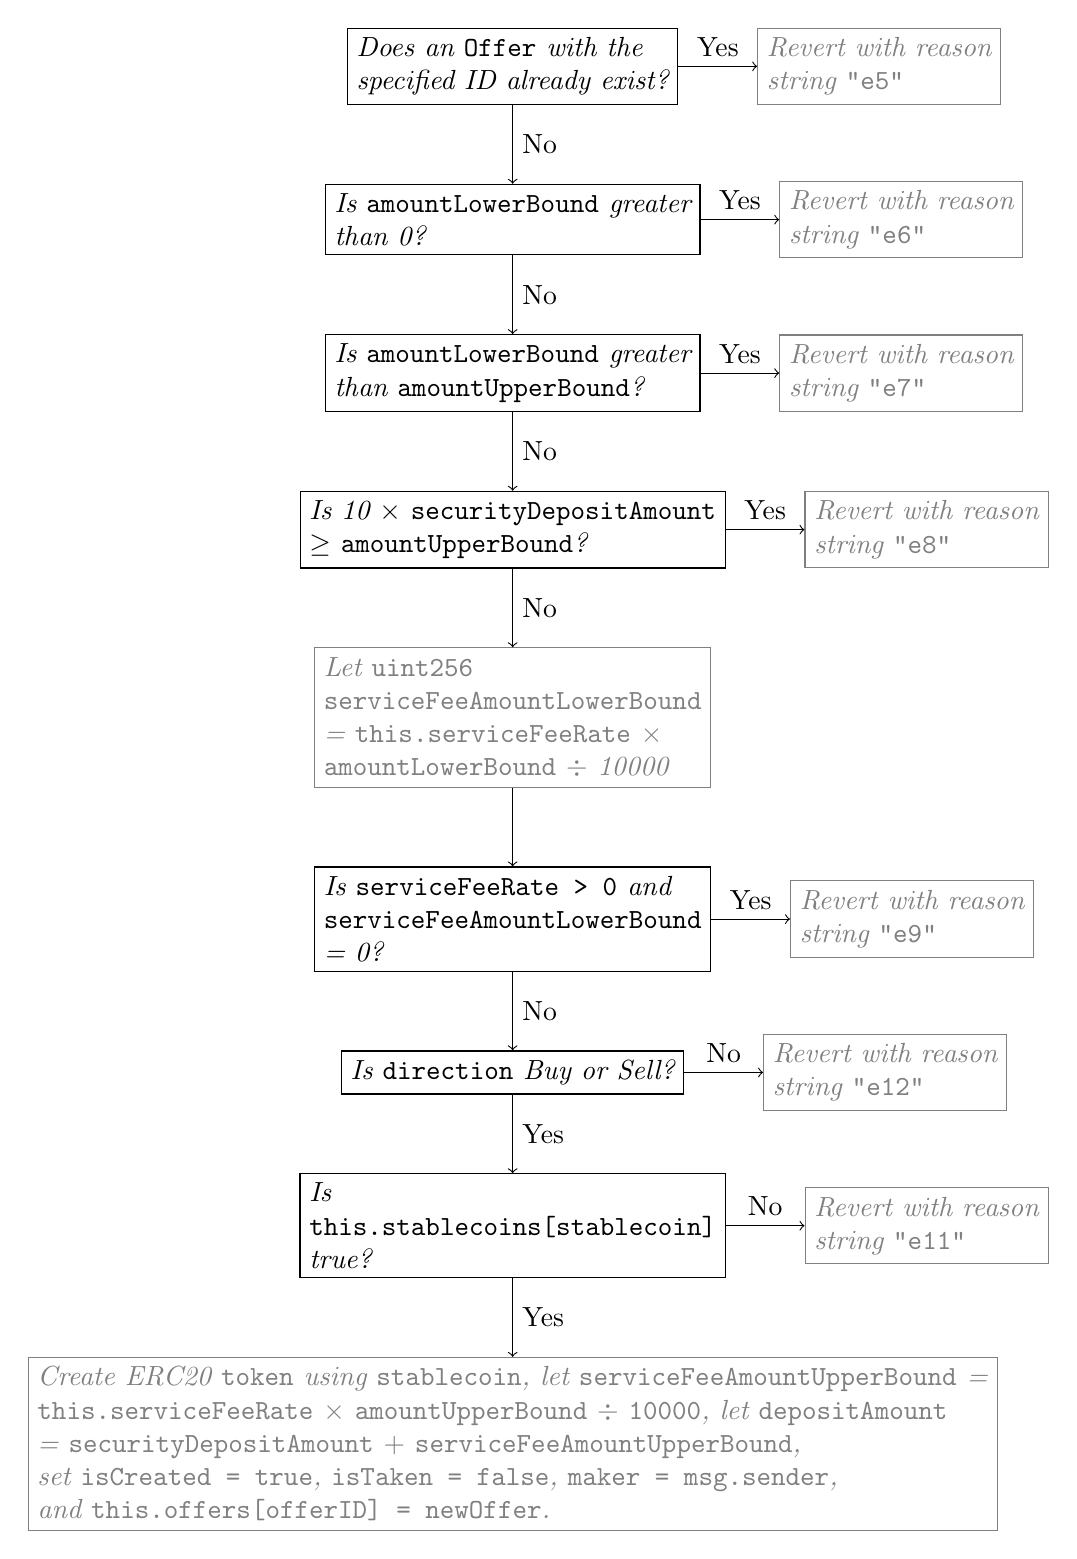
\begin{tikzpicture}[
        question/.style={
            % The shape
            rectangle,
            % The border
            thin,
            draw = black!100,
            % The color
            color = black,
            % Font
            font = \itshape
        },
        action/.style={
            % The shape
            rectangle,
            % The border
            thin,
            draw = gray!100,
            % The color
            color = gray,
            % Font
            font = \itshape
        },
        fail/.style={
            % The shape
            rectangle,
            % The border
            thin,
            draw = red!100,
            % The color
            color = red,
            % Font
            font = \itshape
        },
    ]
        \node (isCreated) [question,align=left] {Does an \verb|Offer| with the \\ specified ID
        already exist?};
        \node (revert_e5) [action,align=left,right=of isCreated] {Revert with reason \\ string
        \verb|"e5"|};
        \path (isCreated) edge[->] node[pos=0.5,above] {Yes} (revert_e5);

        \node (sufficientAmount) [question,align=left,below=of isCreated] {Is
        \verb|amountLowerBound| greater \\ than 0?};
        \path (isCreated) edge[->] node[pos=0.5,right] {No} (sufficientAmount);
        \node (revert_e6) [action,align=left,right=of sufficientAmount] {Revert with reason \\
        string \verb|"e6"|};
        \path (sufficientAmount) edge[->] node[pos=0.5,above] {Yes} (revert_e6);

        \node (properRange) [question,align=left,below=of sufficientAmount ] {Is
        \verb|amountLowerBound| greater \\ than \verb|amountUpperBound|?};
        \path (sufficientAmount) edge[->] node[pos=0.5,right] {No} (properRange);
        \node (revert_e7) [action,align=left,right=of properRange] {Revert with reason \\ string
        \verb|"e7"|};
        \path (properRange) edge[->] node[pos=0.5,above] {Yes} (revert_e7);

        \node (sufficientSecurityDeposit) [question,align=left,below=of properRange] {Is 10 $\times$ \verb|securityDepositAmount| \\ $\geq$ \verb|amountUpperBound|?};
        \path (properRange) edge[->] node[pos=0.5,right] {No} (sufficientSecurityDeposit);
        \node (revert_e8) [action,align=left,right=of sufficientSecurityDeposit] {Revert with reason \\ string \verb|"e8"|};
        \path (sufficientSecurityDeposit) edge[->] node[pos=0.5,above] {Yes} (revert_e8);

        \node (calculateServiceFeeAmntLow) [action,align=left,below=of sufficientSecurityDeposit] {Let \verb|uint256| \\ \verb|serviceFeeAmountLowerBound| \\ = \verb|this.serviceFeeRate| $\times$ \\ \verb|amountLowerBound| $\div$ 10000};
        \path (sufficientSecurityDeposit) edge[->] node[pos=0.5,right] {No} (calculateServiceFeeAmntLow);

        \node (sufficientServiceFee) [question,align=left,below=of calculateServiceFeeAmntLow] {Is \verb|serviceFeeRate > 0| and \\ \verb|serviceFeeAmountLowerBound| \\ = 0?};
        \path (calculateServiceFeeAmntLow) edge[->] (sufficientServiceFee);
        \node (revert_e9) [action,align=left,right=of sufficientServiceFee] {Revert with reason \\ string \verb|"e9"|};
        \path (sufficientServiceFee) edge[->] node[pos=0.5,above] {Yes} (revert_e9);

        \node (validDirection) [question,align=left,below=of sufficientServiceFee] {Is \verb|direction| Buy or Sell?};
        \path (sufficientServiceFee) edge[->] node[pos=0.5,right] {No} (validDirection);
        \node (revert_e12) [action,align=left,right=of validDirection] {Revert with reason \\ string \verb|"e12"|};
        \path (validDirection) edge[->] node[pos=0.5,above] {No} (revert_e12);

        \node (validToken) [question,align=left,below=of validDirection] {Is \\ \verb|this.stablecoins[stablecoin]| \\ true?};
        \path (validDirection) edge[->] node[pos=0.5,right] {Yes} (validToken);
        \node (revert_e11) [action,align=left,right=of validToken] {Revert with reason \\ string \verb|"e11"|};
        \path (validToken) edge[->] node[pos=0.5,above] {No} (revert_e11);

        \node (openOffer) [action,align=left,below=of validToken] {
            Create ERC20 \verb|token| using \verb|stablecoin|, let \verb|serviceFeeAmountUpperBound|
            = \\ \verb|this.serviceFeeRate| $\times$ \verb|amountUpperBound| $\div$ \verb|10000|,
            let \verb|depositAmount| \\ = \verb|securityDepositAmount| $+$
            \verb|serviceFeeAmountUpperBound|, \\ set \verb|isCreated = true|,
            \verb|isTaken = false|, \verb|maker = msg.sender|,\\ and
            \verb|this.offers[offerID] = newOffer|.

        };
        \path (validToken) edge[->] node[pos=0.5,right] {Yes} (openOffer);

    \end{tikzpicture}

    Continued on next page.

    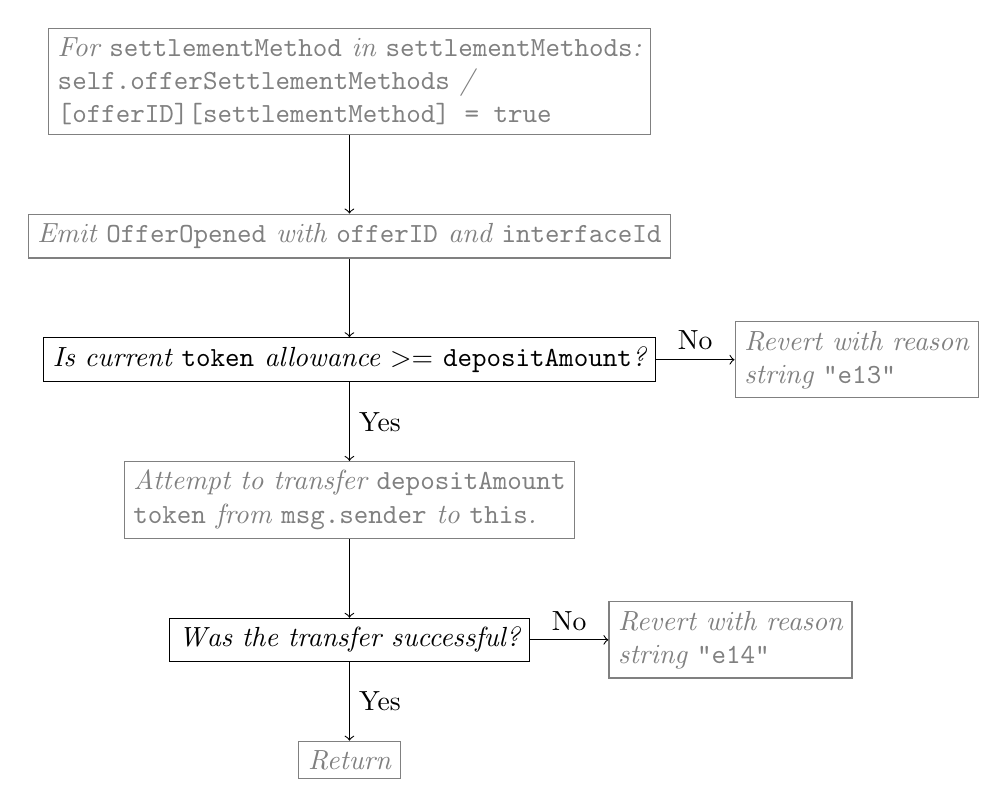
\begin{tikzpicture}[
        question/.style={
            rectangle, thin, draw = black!100, color = black, font = \itshape
        },
        action/.style={
            rectangle, thin, draw = gray!100, color = gray, font = \itshape
        },
    ]
    \node (addSettlementMethods) [action,align=left] {
        For \verb|settlementMethod| in \verb|settlementMethods|: \\
        \verb|self.offerSettlementMethods| / \\
        \verb|[offerID][settlementMethod] = true|
    };

    \node (emitEvent) [action, below=of addSettlementMethods] { Emit \verb|OfferOpened| with \verb|offerID| and \verb|interfaceId| };
    \path (addSettlementMethods) edge[->] (emitEvent);

    \node (verifyAllowance) [question, below=of emitEvent] { Is current \verb|token| allowance $>=$ \verb|depositAmount|? };
    \path (emitEvent) edge[->] (verifyAllowance);
    \node (revert_e13) [action,align=left,right=of verifyAllowance] {Revert with reason \\ string \verb|"e13"|};
    \path (verifyAllowance) edge[->] node[pos=0.5,above] {No} (revert_e13);

    \node (attemptTransfer) [action,align=left,below=of verifyAllowance] { Attempt to transfer \verb|depositAmount| \\ \verb|token| from \verb|msg.sender| to \verb|this|. };
    \path (verifyAllowance) edge[->] node[pos=0.5,right] {Yes} (attemptTransfer);

    \node (verifyTransfer) [question,below=of attemptTransfer] {Was the transfer successful?};
    \path (attemptTransfer) edge[->] (verifyTransfer);
    \node (revert_e14) [action,align=left,right=of verifyTransfer] {Revert with reason \\ string \verb|"e14"|};
    \path (verifyTransfer) edge[->] node[pos=0.5,above] {No} (revert_e14);
    \node (return) [action,below=of verifyTransfer] {Return};
    \path (verifyTransfer) edge[->] node[pos=0.5,right] {Yes} (return);

    \end{tikzpicture}

    \subsubsection*{Taking an Offer}

    An offer taker takes an existing offer by calling the \verb|takeOffer| function.
    This function has the following signature:
    \begin{verbatim}
    takeOffer(bytes16 offerID, Swap newSwap)
    \end{verbatim}
    where \verb|offerID| is a Version-4 UUID and newSwap is a \verb|Swap| struct that is defined as
    follows:
    \begin{longtable}[p]{ |p{2.5cm}|p{4cm}|p{7cm}| }
        \hline
        \multicolumn{3}{|c|}{Swap} \\
        \hline
        Property Type & Property Name & Description \\
        \hline
        bool & isCreated & Used by contract code to check for swap existence, will be set to true by \verb|takeOffer|. \\
        bool & requiresFill & If the maker of this swap is the token seller, this indicates whether the seller has transferred to CommutoSwap the amount of tokens that they are selling.
        If the maker of this swap is not the token seller, this is not used. \\
        address & maker & Identical to \verb|Offer.maker| of the offer being taken. \\
        bytes & makerInterfaceId & Identical to \verb|Offer.interfaceId| of the offer being taken. \\
        address & taker & The taker's address, will be sent to \verb|msg.sender| by \verb|takeOffer|. \\
        bytes & takerInterfaceId & An array of bytes that should be placed in the “recipient” field of
        any message sent to the taker of this offer via Matrix. \\
        address & stablecoin & Identical to \verb|Offer.stablecoin| of the offer being taken. \\
        uint256 & amountLowerBound & Identical to \verb|Offer.amountLowerBound| of the offer being taken. \\
        uint256 & amountUpperBound & Identical to \verb|Offer.amountUpperBound| of the offer being taken. \\
        uint256 & securityDepositAmount & Identical to \verb|Offer.securityDepositAmount| of the offer being taken. \\
        uint256 & takenSwapAmount & The exact amount of tokens that will be exchanged between the maker and the taker.
        Must be such that \verb|amountLowerBound| $\leq$ takenSwapAmount $\leq$ \verb|amountUpperBound|. \\
        uint256 & serviceFeeAmount & Used by contract code, will be set to \verb|Offer.serviceFeeRate| of the offer being taken $\times$ \verb|takenSwapAmount| $\div$ \verb|10000|.\\
        uint256 & serviceFeeRate & Identical to \verb|Offer.serviceFeeRate| of the offer being taken. \\
        SwapDirection & direction & Identical to \verb|Offer.direction| of the offer being taken. \\
        bytes & settlementMethod & A \verb|bytes| value representing the method by which the buyer will send payment for the exchanged tokens.
        Must be equal to one of the elements in the \verb|Offer.settlementMethods| array of the offer being taken. \\
        uint256 & protocolVersion & Identical to \verb|Offer.protocolVersion| of the offer being taken. \\
        bool & isPaymentSent & Indicates whether the buyer has sent payment for tokens purchased.
        Will be set to false by \verb|takeOffer|. \\
        bool & isPaymentReceived & Indicates whether the seller has received payment for tokens sold.
        Will be set to false by \verb|takeOffer|. \\
        bool & hasBuyerClosed & Indicates whether the buyer has closed the swap to reclaim their security deposit (and unused service fee amount, if they are the maker).
        Will be set to false by \verb|takeOffer|. \\
        bool & hasSellerClosed & Indicates whether the seller has closed the swap to reclaim their security deposit (and unused service fee amount, if they are the maker).
        Will be set to false by \verb|takeOffer|. \\
        DisputeRaiser & disputeRaiser & Indicates whether the buyer, seller, or neither has raised a dispute during the swap process.
        Will be set to \verb|NONE| by \verb|takeOffer|. \\
        \hline
    \end{longtable}
    \verb|DisputeRaiser| is an \verb|enum| that is defined as follows:
    \begin{verbatim}
    enum DisputeRaiser  {
        NONE,
        MAKER,
        TAKER
    }
    \end{verbatim}
    The meaning of these values and the use of the \verb|Swap.disputeRaiser| property will be
    described later in this paper.

    When called, \verb|takeOffer| ensures that an Offer with the specified ID already exists and is
    not taken, and validates all the data that it has been passed to ensure that it corresponds with
    the Offer being taken.
    Then this sets a flag on the Offer being taken to indicate this, and adds the new swap to
    \verb|this.swaps|.
    \verb|this.swaps| is a property of the CommutoSwap contract, and is a mapping from
    \verb|bytes16| values to \verb|Swap|s.
    Then this emits an \verb|OfferTaken| event with the ID of the Offer and the interface ID of the
    taker.
    The \verb|OfferTaken| Event has the following signature:
    \begin{verbatim}
    OfferTaken(bytes16 offerID, bytes takerInterfaceId)
    \end{verbatim}
    Then this transfers to itself from the taker an amount of the specified token.
    If the taker is the buyer, this amount is equal to the security deposit plus the exact service
    fee.
    If the taker is the seller, this amount is equal to the security deposit plus the exact service
    fee plus the amount to be sold.
    This process is shown in Figure 1.2.

    %TODO: Add label here
    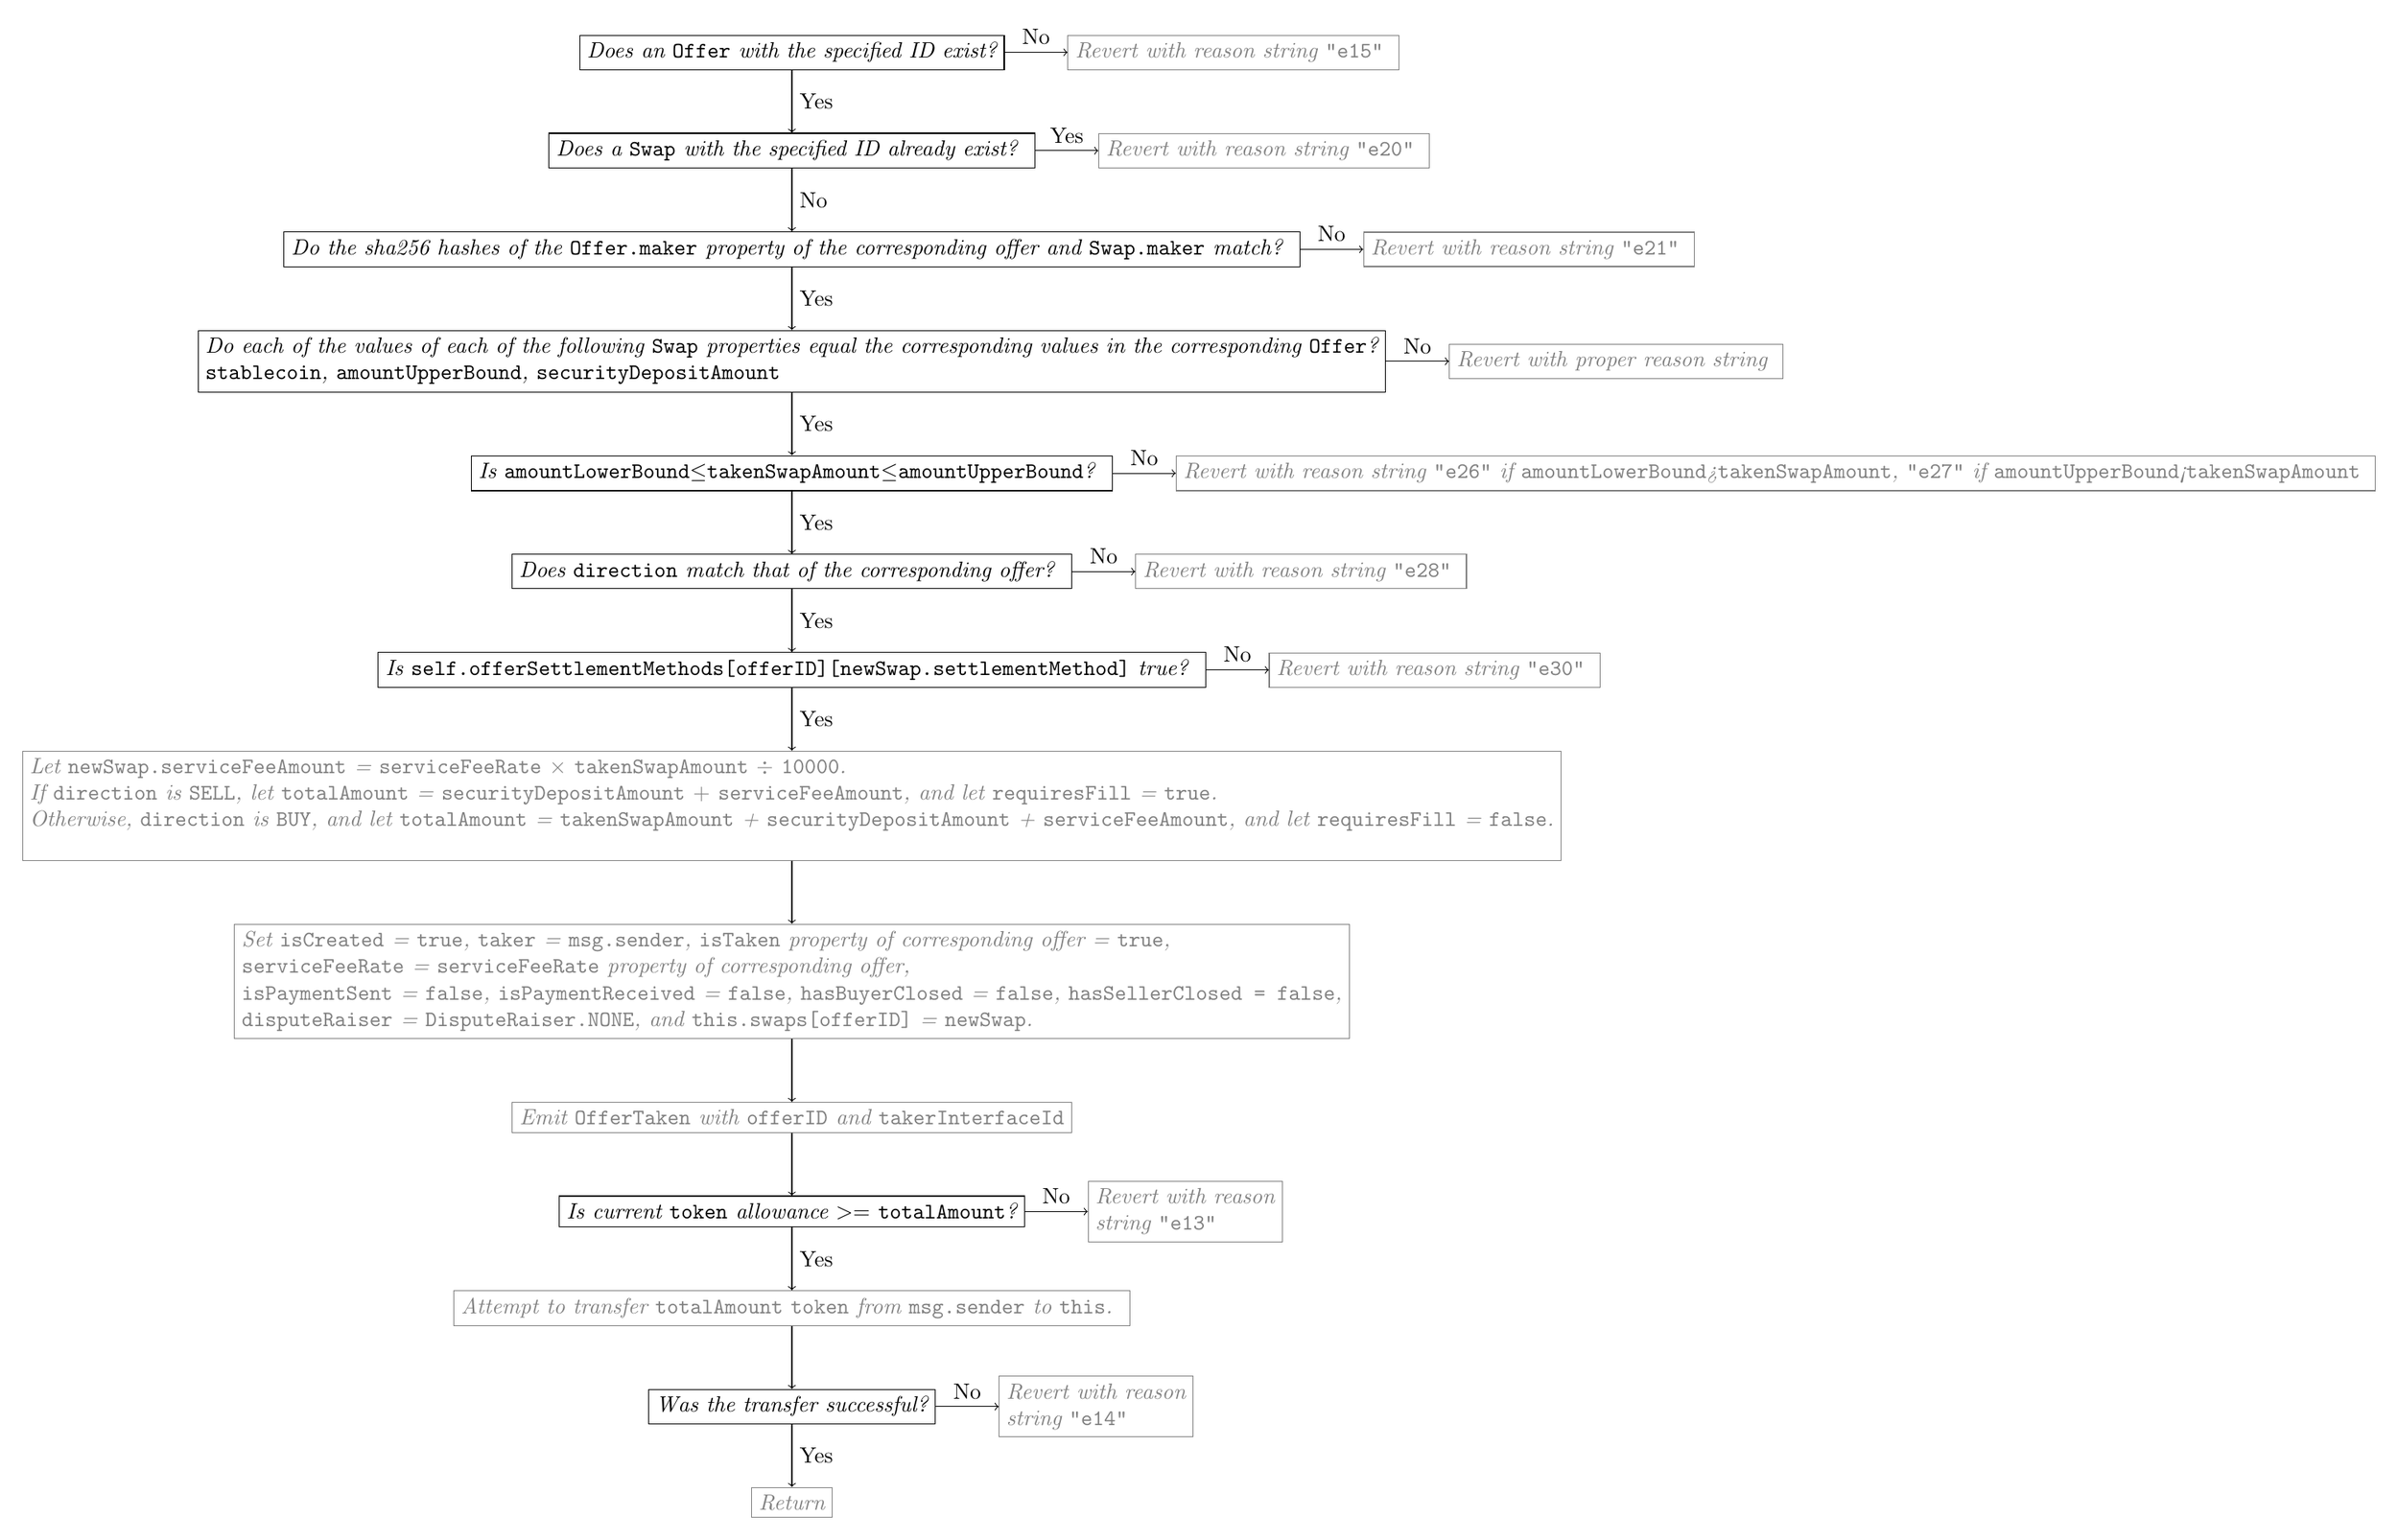
\begin{tikzpicture}[
        question/.style={
            rectangle, thin, draw = black!100, color = black, font = \itshape
        },
        action/.style={
            rectangle, thin, draw = gray!100, color = gray, font = \itshape
        },
    ]
        \node (isCreated) [question,align=left] { Does an \verb|Offer| with the specified ID exist?};
        \node (revert_e15) [action,align=left,right=of isCreated] { Revert with reason string \verb|"e15"| };
        \path (isCreated) edge[->] node[pos=0.5,above] {No} (revert_e15);

        \node (sufficientAmount) [question,align=left,below=of isCreated] { Does a \verb|Swap| with the specified ID already exist? };
        \path (isCreated) edge[->] node[pos=0.5,right] {Yes} (sufficientAmount);
        \node (revert_e20) [action,align=left,right=of sufficientAmount] { Revert with reason string \verb|"e20"| };
        \path (sufficientAmount) edge[->] node[pos=0.5,above] {Yes} (revert_e20);

        \node (matchingMakerID) [question,align=left,below=of sufficientAmount] { Do the sha256 hashes of the \verb|Offer.maker| property of the corresponding offer and \verb|Swap.maker| match? };
        \path (sufficientAmount) edge[->] node[pos=0.5,right] {No} (matchingMakerID);
        \node (revert_e21) [action,align=left,right=of matchingMakerID] { Revert with reason string \verb|"e21"| };
        \path (matchingMakerID) edge[->] node[pos=0.5,above] {No} (revert_e21);

        \node (matchingProperties1) [question,align=left,below=of matchingMakerID] {
            Do each of the values of each of the following \verb|Swap| properties equal the
            corresponding values in the corresponding \verb|Offer|? \\
            \verb|stablecoin|, \verb|amountUpperBound|, \verb|securityDepositAmount|
        };
        \path (matchingMakerID) edge[->] node[pos=0.5,right] {Yes} (matchingProperties1);
        \node (revert_proper1) [action,align=left,right=of matchingProperties1] { Revert with proper reason string };
        \path (matchingProperties1) edge[->] node[pos=0.5,above] {No} (revert_proper1);

        \node (amountInRange) [question,align=left,below=of matchingProperties1] { Is \verb|amountLowerBound|$\leq$\verb|takenSwapAmount|$\leq$\verb|amountUpperBound|? };
        \path (matchingProperties1) edge[->] node[pos=0.5,right] {Yes} (amountInRange);
        \node (revert_e26_e27) [action,align=left,right=of amountInRange] { Revert with reason string \verb|"e26"| if \verb|amountLowerBound|>\verb|takenSwapAmount|, \verb|"e27"| if \verb|amountUpperBound|<\verb|takenSwapAmount| };
        \path (amountInRange) edge[->] node[pos=0.5,above] {No} (revert_e26_e27);

        \node (matchingDirection) [question,align=left,below=of amountInRange] { Does \verb|direction| match that of the corresponding offer? };
        \path (amountInRange) edge[->] node[pos=0.5,right] {Yes} (matchingDirection);
        \node (revert_e28) [action,align=left,right=of matchingDirection] { Revert with reason string \verb|"e28"| };
        \path (matchingDirection) edge[->] node[pos=0.5,above] {No} (revert_e28);

        \node (settlementMethodSupported) [question,align=left,below=of matchingDirection] { Is \verb|self.offerSettlementMethods[offerID][newSwap.settlementMethod]| true? };
        \path (matchingDirection) edge[->] node[pos=0.5,right] {Yes} (settlementMethodSupported);
        \node (revert_e30) [action,align=left,right=of settlementMethodSupported] { Revert with reason string \verb|"e30"| };
        \path (settlementMethodSupported) edge[->] node[pos=0.5,above] {No} (revert_e30);

        \node (calculateAmounts) [action,align=left,below=of settlementMethodSupported] {
            Let \verb|newSwap.serviceFeeAmount| = \verb|serviceFeeRate| $\times$ \verb|takenSwapAmount| $\div$ \verb|10000|. \\
            If \verb|direction| is \verb|SELL|, let \verb|totalAmount| = \verb|securityDepositAmount| $+$ \verb|serviceFeeAmount|, and let \verb|requiresFill| = \verb|true|. \\
            Otherwise, \verb|direction| is \verb|BUY|, and let \verb|totalAmount| = \verb|takenSwapAmount| + \verb|securityDepositAmount| + \verb|serviceFeeAmount|, and let \verb|requiresFill| = \verb|false|. \\
        };
        \path (settlementMethodSupported) edge[->] node[pos=0.5,right] {Yes} (calculateAmounts);

        \node (setValues) [action,align=left,below=of calculateAmounts] {
            Set \verb|isCreated| = \verb|true|, \verb|taker| = \verb|msg.sender|,
            \verb|isTaken| property of corresponding offer = \verb|true|, \\
            \verb|serviceFeeRate| = \verb|serviceFeeRate| property of corresponding offer, \\
            \verb|isPaymentSent| = \verb|false|, \verb|isPaymentReceived| = \verb|false|, \verb|hasBuyerClosed| = \verb|false|, \verb|hasSellerClosed = false|, \\
            \verb|disputeRaiser| = \verb|DisputeRaiser.NONE|, and \verb|this.swaps[offerID]| = \verb|newSwap|.
        };
        \path (calculateAmounts) edge[->] (setValues);

        \node (emitEvent) [action,below=of setValues] {
            Emit \verb|OfferTaken| with \verb|offerID| and \verb|takerInterfaceId|
        };
        \path (setValues) edge[->] (emitEvent);

        \node (verifyAllowance) [question, below=of emitEvent] { Is current \verb|token| allowance $>=$ \verb|totalAmount|? };
        \path (emitEvent) edge[->] (verifyAllowance);
        \node (revert_e13) [action,align=left,right=of verifyAllowance] {Revert with reason \\ string \verb|"e13"|};
        \path (verifyAllowance) edge[->] node[pos=0.5,above] {No} (revert_e13);

        \node (attemptTransfer) [action,align=left,below=of verifyAllowance] { Attempt to transfer \verb|totalAmount| \verb|token| from \verb|msg.sender| to \verb|this|. };
        \path (verifyAllowance) edge[->] node[pos=0.5,right] {Yes}  (attemptTransfer);

        \node (verifyTransfer) [question,below=of attemptTransfer] {Was the transfer successful?};
        \path (attemptTransfer) edge[->] (verifyTransfer);
        \node (revert_e14) [action,align=left,right=of verifyTransfer] {Revert with reason \\ string \verb|"e14"|};
        \path (verifyTransfer) edge[->] node[pos=0.5,above] {No} (revert_e14);
        \node (return) [action,below=of verifyTransfer] {Return};
        \path (verifyTransfer) edge[->] node[pos=0.5,right] {Yes} (return);

    \end{tikzpicture}

    \subsubsection*{Filling a Swap}

    Consider the amount of tokens transferred from a user to CommutoSwap when the user is opening an
    offer to sell tokens.
    Note that this amount is the sum of the security deposit and the maximum service fee amount;
    The actual amount of tokens that the user wishes to sell is not transferred when opening such an
    offer.
    Therefore, when another user takes an offer to sell tokens, the amount of tokens being sold must
    be transferred from the offer maker to CommutoSwap.
    (Note that this is not necessary if the maker is offering to buy tokens, and thus this step is
    skilled in such cases.)
    The maker and seller accomplishes this by calling the \verb|fillSwap| function.
    This function has the following signature:
    \begin{verbatim}
        fillSwap(bytes16 swapID)
    \end{verbatim}
    where \verb|swapID| is the ID of the swap to be filled.

    When called, \verb|fillSwap| ensures that the caller is the maker and seller of the specified
    Swap, and that the Swap has not yet been filled.
    Then this sets a flag on the specified Swap indicating that it has been filled, and then emits a
    \verb|SwapFilled| Event with the ID of the Swap.
    The \verb|SwapFilled| Event has the following signature:
    \begin{verbatim}
    SwapFilled(bytes16 swapID)
    \end{verbatim}
    Finally, this transfers to itself from the maker the exact amount of tokens that the taker is
    buying.
    This process is shown in Figure 1.3.

    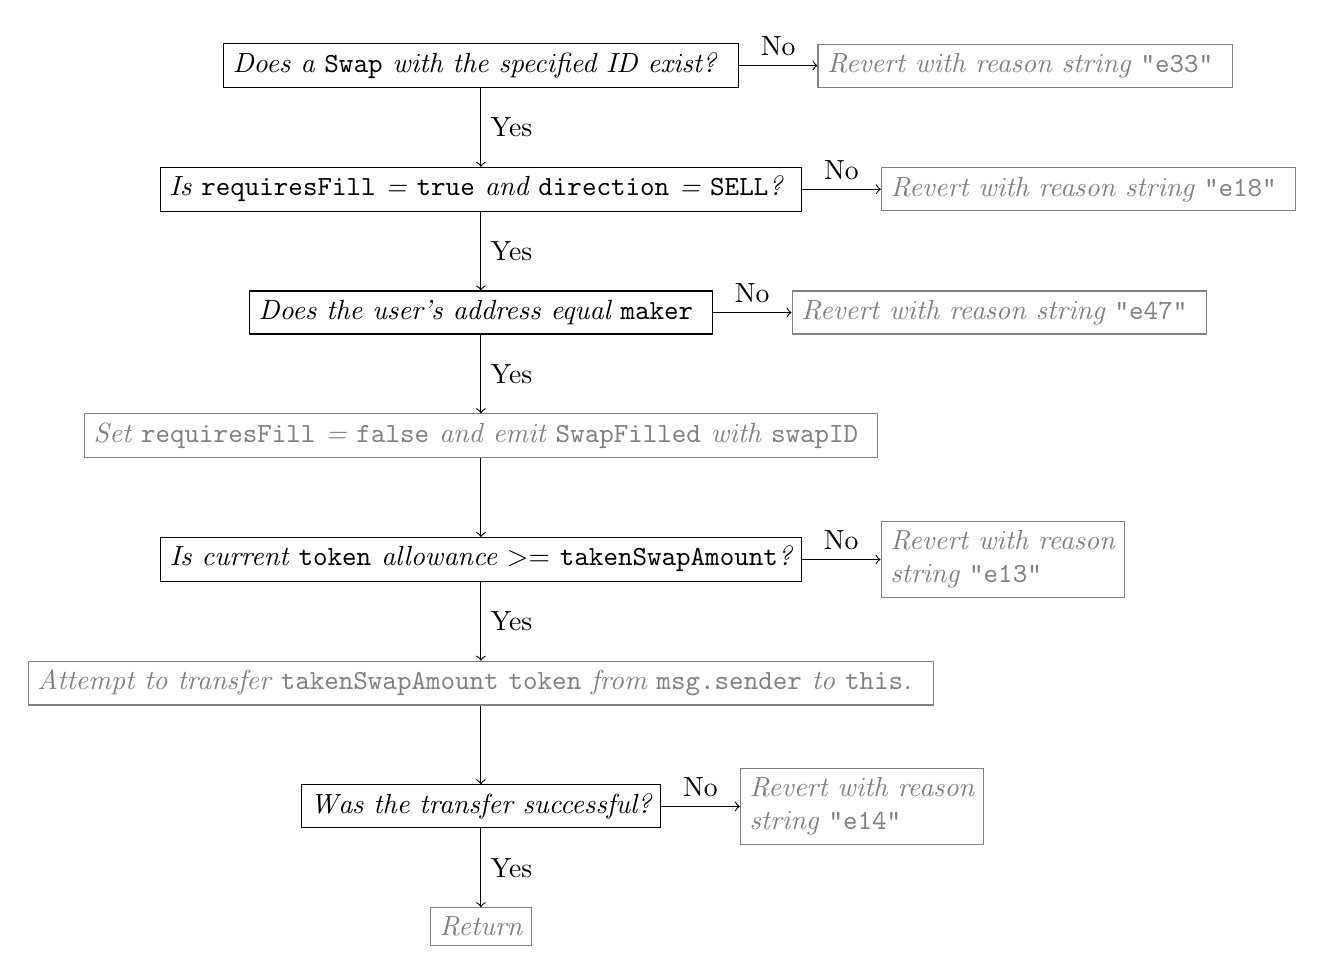
\begin{tikzpicture}[
        question/.style={
            rectangle, thin, draw = black!100, color = black, font = \itshape
        },
        action/.style={
            rectangle, thin, draw = gray!100, color = gray, font = \itshape
        },
    ]
        \node (isCreated) [question,align=left] { Does a \verb|Swap| with the specified ID exist? };
        \node (revert_e33) [action,align=left,right=of isCreated] { Revert with reason string \verb|"e33"| };
        \path (isCreated) edge[->] node[pos=0.5,above] {No} (revert_e33);

        \node (requiresFilling) [question,align=left,below=of isCreated] { Is \verb|requiresFill| = \verb|true| and \verb|direction| = \verb|SELL|? };
        \path (isCreated) edge[->] node[pos=0.5,right] {Yes} (requiresFilling);
        \node (revert_e18) [action,align=left,right=of requiresFilling] { Revert with reason string \verb|"e18"| };
        \path (requiresFilling) edge[->] node[pos=0.5,above] {No} (revert_e18);

        \node (isMaker) [question,align=left,below=of requiresFilling] { Does the user's address equal \verb|maker| };
        \path (requiresFilling) edge[->] node[pos=0.5,right] {Yes} (isMaker);
        \node (revert_e47) [action,align=left,right=of isMaker] { Revert with reason string \verb|"e47"| };
        \path (isMaker) edge[->] node[pos=0.5,above] {No} (revert_e47);

        \node (setAndEmit) [action,align=left,below=of isMaker] { Set \verb|requiresFill| = \verb|false| and emit \verb|SwapFilled| with \verb|swapID| };
        \path (isMaker) edge[->] node[pos=0.5,right] {Yes} (setAndEmit);

        \node (verifyAllowance) [question, below=of setAndEmit] { Is current \verb|token| allowance $>=$ \verb|takenSwapAmount|? };
        \path (setAndEmit) edge[->] (verifyAllowance);
        \node (revert_e13) [action,align=left,right=of verifyAllowance] {Revert with reason \\ string \verb|"e13"|};
        \path (verifyAllowance) edge[->] node[pos=0.5,above] {No} (revert_e13);

        \node (attemptTransfer) [action,align=left,below=of verifyAllowance] { Attempt to transfer \verb|takenSwapAmount| \verb|token| from \verb|msg.sender| to \verb|this|. };
        \path (verifyAllowance) edge[->] node[pos=0.5,right] {Yes} (attemptTransfer);

        \node (verifyTransfer) [question,below=of attemptTransfer] {Was the transfer successful?};
        \path (attemptTransfer) edge[->] (verifyTransfer);
        \node (revert_e14) [action,align=left,right=of verifyTransfer] {Revert with reason \\ string \verb|"e14"|};
        \path (verifyTransfer) edge[->] node[pos=0.5,above] {No} (revert_e14);
        \node (return) [action,below=of verifyTransfer] {Return};
        \path (verifyTransfer) edge[->] node[pos=0.5,right] {Yes} (return);

    \end{tikzpicture}

    \subsubsection*{Sending Payment}

    Now the token seller and buyer must exchange whatever information is necessary for the buyer to
    send payment to the seller.
    This will be accomplished via Matrix, and the precise details of this information exchanging
    process are described later in this document.
    Once said information is exchanged, the token buyer must send payment to the seller using the
    provided details.
    Then the buyer notifies the seller that this has been done by calling the
    \verb|reportPaymentSent| function.
    This function has the following signature:
    \begin{verbatim}
        reportPaymentSent(bytes16 swapID)
    \end{verbatim}

    When called, \verb|reportPaymentSent| ensures that the the Swap does not need to be filled by
    calling \verb|fillSwap|, that \verb|reportPaymentSent| has not yet been called for the specified
    Swap, that the caller is the buyer, and that the specified Swap is not disputed (Disputed Swaps
    are described later in this document.) Then this sets a flag indicating that
    \verb|reportPaymentSent| has been called and emits a \verb|PaymentSent| event with the ID of the
    Swap.
    The \verb|PaymentSent| Event has the following signature:
    \begin{verbatim}
    PaymentSent(bytes16 swapID)
    \end{verbatim}
    This process is shown in Figure 1.4.

    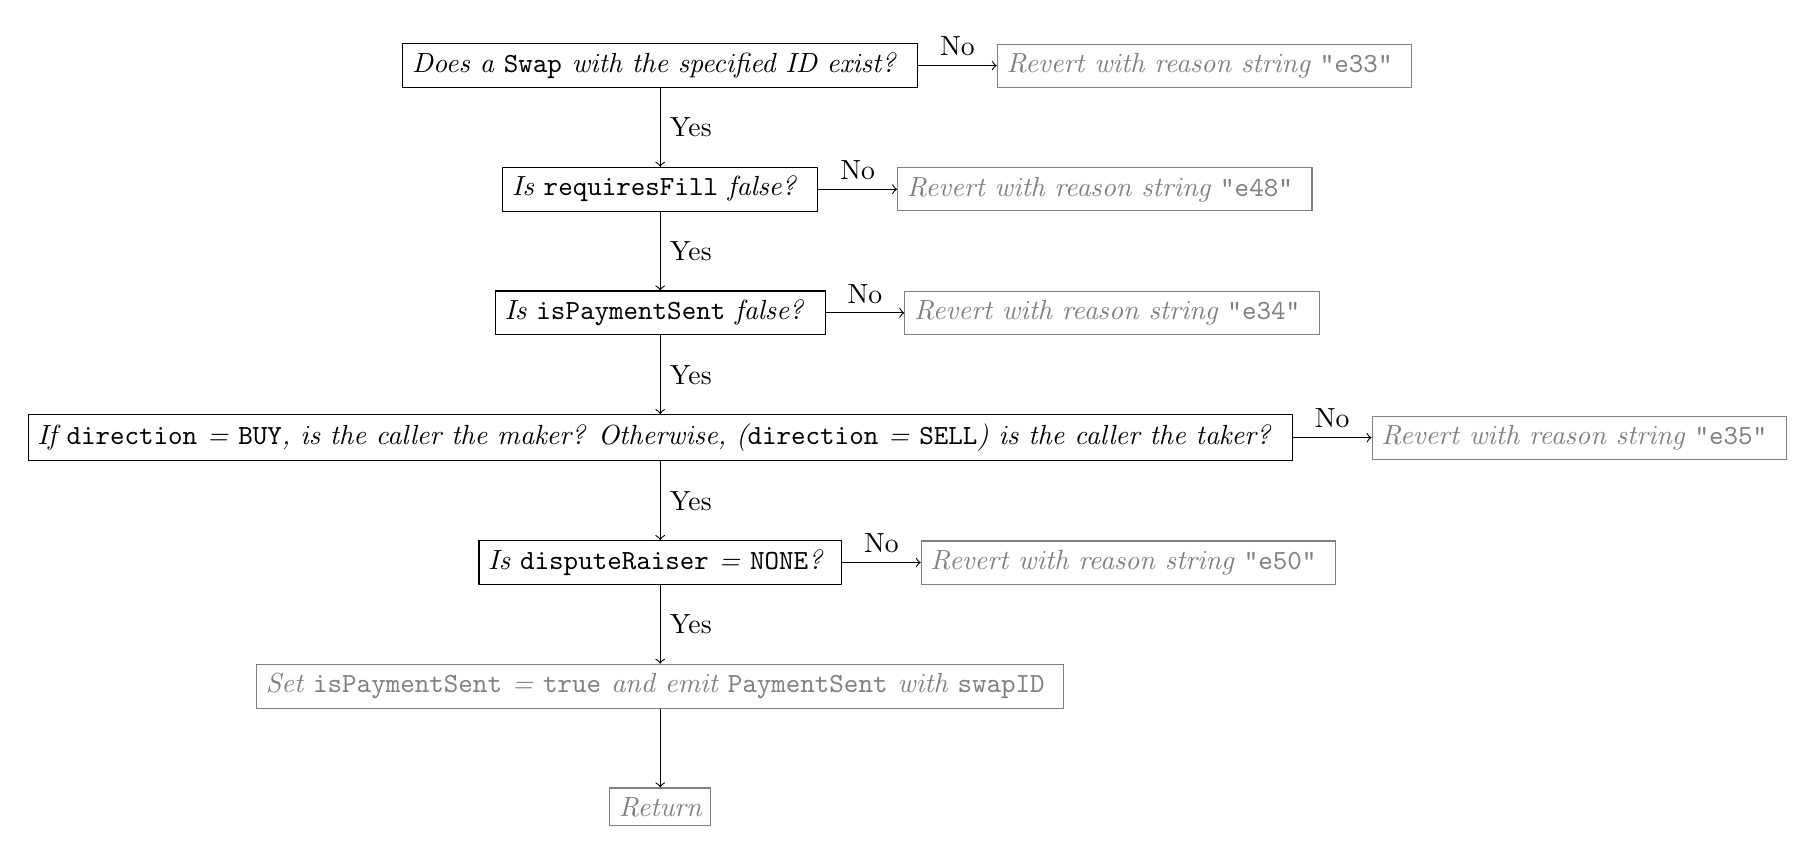
\begin{tikzpicture}[
        question/.style={
            rectangle, thin, draw = black!100, color = black, font = \itshape
        },
        action/.style={
            rectangle, thin, draw = gray!100, color = gray, font = \itshape
        },
    ]
        \node (isCreated) [question,align=left] { Does a \verb|Swap| with the specified ID exist? };
        \node (revert_e33) [action,align=left,right=of isCreated] { Revert with reason string \verb|"e33"| };
        \path (isCreated) edge[->] node[pos=0.5,above] {No} (revert_e33);

        \node (requiresFilling) [question,align=left,below=of isCreated] { Is \verb|requiresFill| false? };
        \path (isCreated) edge[->] node[pos=0.5,right] {Yes} (requiresFilling);
        \node (revert_e48) [action,align=left,right=of requiresFilling] { Revert with reason string \verb|"e48"| };
        \path (requiresFilling) edge[->] node[pos=0.5,above] {No} (revert_e48);

        \node (isPaymentSent) [question,align=left,below=of requiresFilling] { Is \verb|isPaymentSent| false? };
        \path (requiresFilling) edge[->] node[pos=0.5,right] {Yes} (isPaymentSent);
        \node (revert_e34) [action,align=left,right=of isPaymentSent] { Revert with reason string \verb|"e34"| };
        \path (isPaymentSent) edge[->] node[pos=0.5,above] {No} (revert_e34);

        \node (isUserBuyer) [question,align=left,below=of isPaymentSent] { If \verb|direction| = \verb|BUY|, is the caller the maker? Otherwise, (\verb|direction| = \verb|SELL|) is the caller the taker? };
        \path (isPaymentSent) edge[->] node[pos=0.5,right] {Yes} (isUserBuyer);
        \node (revert_e35) [action,align=left,right=of isUserBuyer] { Revert with reason string \verb|"e35"| };
        \path (isUserBuyer) edge[->] node[pos=0.5,above] {No} (revert_e35);

        \node (isDisputed) [question,align=left,below=of isUserBuyer] { Is \verb|disputeRaiser| = \verb|NONE|? };
        \path (isUserBuyer) edge[->] node[pos=0.5,right] {Yes} (isDisputed);
        \node (revert_e50) [action,align=left,right=of isDisputed] { Revert with reason string \verb|"e50"| };
        \path (isDisputed) edge[->] node[pos=0.5,above] {No} (revert_e50);

        \node (setAndEmit) [action,align=left,below=of isDisputed] { Set \verb|isPaymentSent| = \verb|true| and emit \verb|PaymentSent| with \verb|swapID| };
        \path (isDisputed) edge[->] node[pos=0.5,right] {Yes} (setAndEmit);
        \node (return) [action, below=of setAndEmit] {Return};
        \path (setAndEmit) edge[->] (return);

    \end{tikzpicture}

    \subsubsection*{Receiving Payment}

    Once the token seller receives the payment that has been sent by the buyer, the seller must
    notify the buyer by calling the \verb|reportPaymentReceived| function.
    This function has the following signature:
    \begin{verbatim}
        reportPaymentReceived(bytes16 swapID)
    \end{verbatim}

    When called, \verb|reportPaymentReceived| ensures that the buyer in the specified Swap has
    already called \verb|reportPaymentSent|, that \verb|reportPaymentReceived| has not yet been
    called for the specified Swap, that the caller is the seller, and that the specified Swap is not
    disputed.
    Then this sets a flag indicating that \verb|reportPaymentReceived| has been called and emits a
    \verb|PaymentReceived| Event with the ID of the specified Swap.
    The \verb|PaymentReceived| Event has the following signature:
    \begin{verbatim}
    PaymentReceived(bytes16 swapID)
    \end{verbatim}
    This process is shown in Figure 1.5.

    \begin{tikzpicture}[
        question/.style={
            rectangle, thin, draw = black!100, color = black, font = \itshape
        },
        action/.style={
            rectangle, thin, draw = gray!100, color = gray, font = \itshape
        },
    ]
        \node (isCreated) [question,align=left] { Does a \verb|Swap| with the specified ID exist? };
        \node (revert_e33) [action,align=left,right=of isCreated] { Revert with reason string \verb|"e33"| };
        \path (isCreated) edge[->] node[pos=0.5,above] {No} (revert_e33);

        \node (isPaymentSent) [question,align=left,below=of isCreated] { Is \verb|isPaymentSent| true? };
        \path (isCreated) edge[->] node[pos=0.5,right] {Yes} (requiresFilling);
        \node (revert_e37) [action,align=left,right=of isPaymentSent] { Revert with reason string \verb|"e37"| };
        \path (isPaymentSent) edge[->] node[pos=0.5,above] {No} (revert_e37);

        \node (isPaymentReceived) [question,align=left,below=of isPaymentSent] { Is \verb|isPaymentReceived| false? };
        \path (isPaymentSent) edge[->] node[pos=0.5,right] {Yes} (isPaymentReceived);
        \node (revert_e38) [action,align=left,right=of isPaymentReceived] { Revert with reason string \verb|"e38"| };
        \path (isPaymentReceived) edge[->] node[pos=0.5,above] {No} (revert_e38);

        \node (isUserSeller) [question,align=left,below=of isPaymentReceived] { If \verb|direction| = \verb|BUY|, is the caller the taker? Otherwise, (\verb|direction| = \verb|SELL|) is the caller the maker? };
        \path (isPaymentReceived) edge[->] node[pos=0.5,right] {Yes} (isUserSeller);
        \node (revert_e39) [action,align=left,right=of isUserSeller] { Revert with reason string \verb|"e39"| };
        \path (isUserSeller) edge[->] node[pos=0.5,above] {No} (revert_e39);

        \node (isDisputed) [question,align=left,below=of isUserSeller] { Is \verb|disputeRaiser| = \verb|NONE|? };
        \path (isUserSeller) edge[->] node[pos=0.5,right] {Yes} (isDisputed);
        \node (revert_e51) [action,align=left,right=of isDisputed] { Revert with reason string \verb|"e51"| };
        \path (isDisputed) edge[->] node[pos=0.5,above] {No} (revert_e51);

        \node (setAndEmit) [action,align=left,below=of isDisputed] { Set \verb|isPaymentReceived| = \verb|true| and emit \verb|PaymentReceived| with \verb|swapID| };
        \path (isDisputed) edge[->] node[pos=0.5,right] {Yes} (setAndEmit);
        \node (return) [action, below=of setAndEmit] {Return};
        \path (setAndEmit) edge[->] (return);

    \end{tikzpicture}

    \verb|PaymentSent| is an Event with the following signature:
    \begin{verbatim}
        PaymentReceived(bytes16 swapID)
    \end{verbatim}

    \subsubsection*{Closing the Swap}

    Now that the token seller has received payment from the buyer, both the buyer and the seller
    must close the swap by calling the \verb|closeSwap| function.
    This function has the following signature:
    \begin{verbatim}
        closeSwap(bytes16 swapID)
    \end{verbatim}

    When called, \verb|closeSwap| ensures that \verb|reportPaymentReceived| has been called for the
    swap, and that the specified Swap is not disputed.
    It transfer's the caller's service fee to \verb|this.primaryTimelock|, which is a property of
    the CommutoSwap contract of type \verb|address|, to which all service fees are sent.
    This property is also used by administration and governance-related code, which is described
    later in this document.
    If the caller is the buyer and taker, this will ensure that they have not already called
    \verb|closeSwap| for the Swap, and then will refund their security deposit and will transfer the
    to them the tokens they bought.
    If the caller is the buyer and maker, this will ensure that they have not already called
    \verb|closeSwap| for the Swap, and then will refund their security deposit and transfer to them
    the tokens they bought and the remainder of the maximum service fee (if any) that they
    transferred to CommutoSwap when opening the offer.
    If the caller is the seller and taker, this will ensure that they have not already called
    \verb|closeSwap| for the swap, and then will refund their security deposit.
    If the caller is the seller and maker, this will ensure that they have not already called
    \verb|closeSwap| for the swap, and then will refund their security deposit and will transfer to
    them the remainder of the maximum service fee (if any) that they transferred to CommutoSwap when
    opening the offer.
    If the caller is the buyer, this will then emit a BuyerClosed Event.
    If the caller is the seller, this will then emit a SellerClosed Event.
    Both specify the Swap ID\@.
    These Events have the following signature:
    \begin{verbatim}
        BuyerClosed(bytes16 swapID), SellerClosed(bytes16 swapID)
    \end{verbatim}
    Once buyer and seller have both requested Swap closure, the Swap is completely closed.
    This process is shown in Figure 1.6.

    \begin{tikzpicture}[
        question/.style={
            rectangle, thin, draw = black!100, color = black, font = \itshape
        },
        action/.style={
            rectangle, thin, draw = gray!100, color = gray, font = \itshape
        },
    ]
        \node (isCreated) [question,align=left] { Does a \verb|Swap| with the specified ID exist? };
        \node (revert_e33) [action,align=left,right=of isCreated] { Revert with reason string \verb|"e33"| };
        \path (isCreated) edge[->] node[pos=0.5,above] {No} (revert_e33);

        \node (isPaymentReceived) [question,align=left,below=of isCreated] { Is \verb|isPaymentReceived| true? };
        \path (isCreated) edge[->] node[pos=0.5,right] {Yes} (requiresFilling);
        \node (revert_e40) [action,align=left,right=of isPaymentReceived] { Revert with reason string \verb|"e40"| };
        \path (isPaymentReceived) edge[->] node[pos=0.5,above] {No} (revert_e40);

        \node (isDisputed) [question,align=left,below=of isPaymentReceived] { Is \verb|disputeRaiser| = \verb|NONE|? };
        \path (isPaymentReceived) edge[->] node[pos=0.5,right] {Yes} (isDisputed);
        \node (revert_e52) [action,align=left,right=of isDisputed] { Revert with reason string \verb|"e52"| };
        \path (isDisputed) edge[->] node[pos=0.5,above] {No} (revert_e52);

        \node (isBuyerAndTaker) [question,align=left,below=of isDisputed] { Is the caller the buyer and taker? };
        \path (isDisputed) edge[->] node[pos=0.5,right] {Yes} (isBuyerAndTaker);
        \node (hasBuyerAndTakerClosed) [question,align=left,right=of isBuyerAndTaker] { Has the buyer already closed the swap? };
        \path (isBuyerAndTaker) edge[->] node[pos=0.5,above] {Yes} (hasBuyerAndTakerClosed);
        \node (revert_e41_BAT) [action,align=left,below=of hasBuyerAndTakerClosed] { Revert with reason string \verb|"e41"| };
        \path (hasBuyerAndTakerClosed) edge[->] node[pos=0.5,right] {Yes} (revert_e41_BAT);
        \node (calcSetEmitAttemptForBuyerAndTaker) [action,align=left,right=of hasBuyerAndTakerClosed] { Let \verb|returnAmount| = \verb|securityDepositAmount| $+$ \verb|takenSwapAmount|, set \verb|hasBuyerClosed| = \verb|true|, and emit \verb|BuyerClosed| with \verb|swapID|. Then attempt to transfer \verb|returnAmount| of \verb|stablecoin| to \verb|taker|. };
        \path (hasBuyerAndTakerClosed) edge[->] node[pos=0.5,above] {No} (calcSetEmitAttemptForBuyerAndTaker);

        \node (isBuyerAndMaker) [question,align=left,below=25mm of isBuyerAndTaker] { Is the caller the buyer and maker? };
        \path (isBuyerAndTaker) edge[->] node[pos=0.5,right] {No} (isBuyerAndMaker);
        \node (hasBuyerAndMakerClosed) [question,align=left,right=of isBuyerAndMaker] { Has the buyer already closed the swap? };
        \path (isBuyerAndMaker) edge[->] node[pos=0.5,above] {Yes} (hasBuyerAndMakerClosed);
        \node (revert_e41_BAM) [action,align=left,below=of hasBuyerAndMakerClosed] { Revert with reason string \verb|"e41"| };
        \path (hasBuyerAndMakerClosed) edge[->] node[pos=0.5,right] {Yes} (revert_e41_BAM);
        \node (calcSetEmitAttemptForBuyerAndMaker) [action,align=left,right=of hasBuyerAndMakerClosed] { Let \verb|serviceFeeAmountUpperBound| = \verb|serviceFeeRate| $\times$ \verb|amountUpperBound| $\div 10000$, \verb|returnAmount| = \verb|securityDepositAmount| $+$ \verb|takenSwapAmount| $+$ \verb|serviceFeeAmountUpperBound| $-$ \verb|serviceFeeAmount|, set \verb|hasBuyerClosed| = \verb|true|, and emit \verb|BuyerClosed| with \verb|swapID|. Then attempt to transfer \verb|returnAmount| of \verb|stablecoin| to \verb|maker|. };
        \path (hasBuyerAndMakerClosed) edge[->] node[pos=0.5,above] {No} (calcSetEmitAttemptForBuyerAndMaker);

        \node (isSellerAndTaker) [question,align=left,below=25mm of isBuyerAndMaker] { Is the caller the seller and taker? };
        \path (isBuyerAndMaker) edge[->] node[pos=0.5,right] {No} (isSellerAndTaker);
        \node (hasSellerAndTakerClosed) [question,align=left,right=of isSellerAndTaker] { Has the seller already closed the swap? };
        \path (isSellerAndTaker) edge[->] node[pos=0.5,above] {Yes} (hasSellerAndTakerClosed);
        \node (revert_e43_SAT) [action,align=left,below=of hasSellerAndTakerClosed] { Revert with reason string \verb|"e43"| };
        \path (hasSellerAndTakerClosed) edge[->] node[pos=0.5,right] {Yes} (revert_e43_SAT);
        \node (calcSetEmitAttemptForSellerAndTaker) [action,align=left,right=of hasSellerAndTakerClosed] { Let \verb|returnAmount| = \verb|securityDepositAmount|, set \verb|hasSellerClosed| = \verb|true|, and emit \verb|SellerClosed| with \verb|swapID|. Then attempt to transfer \verb|returnAmount| of \verb|stablecoin| to \verb|taker|. };
        \path (hasSellerAndTakerClosed) edge[->] node[pos=0.5,above] {No} (calcSetEmitAttemptForSellerAndTaker);

        \node (isSellerAndMaker) [question,align=left,below=25mm of isSellerAndTaker] { Is the caller the seller and maker? };
        \path (isSellerAndTaker) edge[->] node[pos=0.5,right] {No} (isSellerAndMaker);
        \node (hasSellerAndMakerClosed) [question,align=left,right=of isSellerAndMaker] { Has the seller already closed the swap? };
        \path (isSellerAndMaker) edge[->] node[pos=0.5,above] {Yes} (hasSellerAndMakerClosed);
        \node (revert_e43_SAM) [action,align=left,below=of hasSellerAndMakerClosed] { Revert with reason string \verb|"e43"| };
        \path (hasSellerAndMakerClosed) edge[->] node[pos=0.5,right] {Yes} (revert_e43_SAM);
        \node (calcSetEmitAttemptForSellerAndMaker) [action,align=left,right=of hasSellerAndMakerClosed] { Let \verb|serviceFeeAmountUpperBound| = \verb|serviceFeeRate| $\times$ \verb|amountUpperBound| $\div 10000$, \verb|returnAmount| = \verb|securityDepositAmount| $+$ \verb|serviceFeeAmountUpperBound| $-$ \verb|serviceFeeAmount|, set \verb|hasSellerClosed| = \verb|true|, and emit \verb|SellerClosed| with \verb|swapID|. Then attempt to transfer \verb|returnAmount| of \verb|stablecoin| to \verb|maker|. };
        \path (hasSellerAndMakerClosed) edge[->] node[pos=0.5,above] {No} (calcSetEmitAttemptForSellerAndMaker);

        \node (verifyTransfer) [question, below=25mm of isSellerAndMaker] {Was the transfer successful?};
        \node (revert_e14) [action,align=left,right=of verifyTransfer] {Revert with reason \\ string \verb|"e14"|};
        %TODO: path from transfer attempt nodes to verifyTransfer here
        \path (verifyTransfer) edge[->] node[pos=0.5,above] {No} (revert_e14);

        \node (attemptServiceFeeTransfer) [action,align=left,below=of verifyTransfer] { Attempt to transfer \verb|serviceFeeAmount| \verb|token| to \verb|this.primaryTimelock|. };
        \node (primaryTimelockNote) [align=left,right=of attemptServiceFeeTransfer] { \verb|this.primaryTimelock| will be explained later in this document. };
        \path (verifyTransfer) edge[->] node[pos=0.5,right] {Yes} (attemptServiceFeeTransfer);

        \node (verifyServiceFeeTransfer) [question,below=of attemptServiceFeeTransfer] {Was the transfer successful?};
        \path (attemptServiceFeeTransfer) edge[->] (verifyServiceFeeTransfer);
        \node (revert_e42) [action,align=left,right=of verifyServiceFeeTransfer] {Revert with reason string \verb|"e42"|};
        \path (verifyServiceFeeTransfer) edge[->] node[pos=0.5,above] {No} (revert_e42);

        \node (return) [action,below=of verifyServiceFeeTransfer] {Return};
        \path (verifyServiceFeeTransfer) edge[->] node[pos=0.5,right] {Yes} (return);

    \end{tikzpicture}

    \subsection*{Editing an Offer}

    A maker of an Offer may wish to change the settlement methods by which they are willing to
    send/receive payment for that particular Offer.
    If the Offer has not yet been taken, they may do this by calling the \verb|editOffer| function.
    This function has the following signature:
    \begin{verbatim}
    editOffer(bytes16 offerID, Offer editedOffer)
    \end{verbatim}
    where \verb|offerID| is ID of the Offer to be edited and \verb|editedOffer| is an \verb|Offer|
    struct as previously defined, the \verb|settlementMethods| property of which contains the
    maker's new settlement methods for the Offer, which will completely replace the Offer's current
    on-chain settlement methods.

    When called, \verb|editOffer| ensures that an Offer with the specified ID exists and is not
    taken, and that the caller is the maker of the specified Offer.
    Then, within the \verb|bytes -> bool| mapping that maps supported settlement methods to
    \verb|true| (which is the inner mapping to which the nested mapping
    \verb|this.offerSettlementMethods| maps \verb|offerID|) this maps all currently supported
    settlement methods to \verb|false|.
    Then, within the same mapping, this maps all settlement methods specified in
    \verb|editedOffer.settlementMethods| to \verb|true|.
    Finally, this updates the value of the Offer's \verb|settlementMethods| with the contents of
    \verb|editedOffer.settlementMethods|, and emits an \verb|OfferEdited| event, specifying the
    Offer ID\@.
    The \verb|OfferEdited| Event has the following signature:
    \begin{verbatim}
    OfferEdited(bytes16 offerID)
    \end{verbatim}

    \subsection*{Cancelling an Offer}

    A maker of an Offer may wish to cancel that particular Offer.
    If the Offer has not yet been taken, they may do this by calling the \verb|cancelOffer|
    function.
    This function has the following signature:
    \begin{verbatim}
    cancelOffer(bytes16 offerID)
    \end{verbatim}
    where \verb|offerID|  is the ID of the Offer to be canceled.

    When called, \verb|cancelOffer| ensures that an Offer with the specified ID exists and is not
    taken, and that the caller is the maker of the specified Offer.
    Then, this deletes the specified Offer from \verb|this.offers|, and within the
    \verb|bytes -> bool| mapping that maps supported settlement methods for this Offer to
    \verb|true| (which is the inner mapping to which the nested mapping
    \verb|this.offerSettlementMethods| maps \verb|offerID|) this maps all the Offer's supported
    settlement methods to \verb|false|.
    Finally, this emits an \verb|OfferCanceled| event, specifying the Offer ID\@, and returns to the
    maker an amount of the specified token for the Offer being canceled equal to the sum of the
    security deposit and maximum service fee amount.
    The \verb|OfferCanceled| Event has the following signature:
    \begin{verbatim}
    OfferCanceled(bytes16 offerID)
    \end{verbatim}

    \subsection*{Dispute Process}
    In the process described above, both the buyer and seller have opportunities to misbehave and
    attempt to obtain payment from the other party without sending payment themselves.
    Additionally, other issues may arise during the process, such as the buyer becoming unable to
    send payment, or the seller becoming unable to receive payment.
    In the event of such issues, users can raise a dispute to request intervention from dispute
    agents, in order to claim whatever tokens or payment are rightly theirs.

    Dispute agents are unbiased, bonded 3rd parties who hear arguments from both the buyer and
    seller concerning what went wrong during the swap, and they should determine who should receive
    the tokens still held by CommutoSwap for the swap.
    CommutoSwap shall have a property named \verb|activeDisputeAgents| of type \verb|address[]|,
    which contains the address of every current/active dispute agent, and a property named
    \verb|disputeAgents| that is a mapping from \verb|address| to \verb|bool| values.
    Every \verb|address| in \verb|activeDisputeAgents| should be mapped to \verb|true| in
    \verb|disputeAgents|, and all other \verb|address|es should be mapped to \verb|false|.
    CommutoSwap shall have a property named \verb|disputes| that is a mapping from \verb|bytes16|
    values to \verb|Dispute| structs.
    This is used to map the IDs of disputed Swaps to the corresponding \verb|Dispute| struct.
    %TODO: include Dispute struct description here
    The \verb|Dispute| struct is defined as follows:
    \begin{longtable}[p]{ |p{2.5cm}|p{4cm}|p{7cm}| }

    \end{longtable}

    In the following description, a ``swapper'' is defined as either the maker of an Offer that has
    been taken, or the taker of an Offer.

    \subsubsection*{Raising a Dispute}
    A swapper raises a dispute by calling the \verb|raiseDispute| function.
    This function has the following signature:
    \begin{verbatim}
    raiseDispute(
        bytes16 swapID,
        address disputeAgent0,
        address disputeAgent1,
        address disputeAgent2
    )
    \end{verbatim}
    where \verb|swapID| is the ID of the Swap to be disputed, and the remaining three arguments are
    unique \verb|address|es that exist in CommutoSwap's \verb|activeDisputeAgents| property.

    When called, \verb|raiseDispute| sets the \verb|disputeRaiser| property of the Swap with the
    specified ID to indicate whether the caller is the maker or the taker of the swap.
    Then, in the \verb|Dispute| to which \verb|swapID| is mapped in CommutoSwap's \verb|disputes|
    property, this sets the \verb|disputeRaisedBlockNum| property to the current block number, and
    the dispute agent addresses to those specified by the caller.
    Finally, this emits a \verb|DisputeRaised| event, specifying the Swap's ID and the three
    addresses supplied by the caller.
    The \verb|DisputeRaised| event has the following signature:
    \begin{verbatim}
    DisputeRaised(
        bytes16 swapID,
        address disputeAgent0,
        address disputeAgent1,
        address disputeAgent2
    )
    \end{verbatim}

    \subsubsection*{Proposing a Resolution}
    Using a Commuto Interface, both the maker and the taker communicate with the dispute agents and
    explain the circumstances of the dispute (which may involve problems sending or receiving
    payment, an unresponsive peer, or other reason.) Similarly, the dispute agents communicate with
    each other to determine a resolution.
    The dispute agents have one week to determine such a resolution.
    They do this by indicating the amount of tokens currently being held by CommutoSwap for the
    disputed Swap in question that the buyer and seller should receive.
    Then each dispute agent calls the \verb|proposeResolution| function, passing those amounts.
    This function has the following signature:
    \begin{verbatim}
    proposeResolution(
        bytes16 swapID,
        uint256 makerPayout,
        uint256 takerPayout,
        uint256 confiscationPayout
    )
    \end{verbatim}
    where \verb|swapID| is the ID of the disputed Swap for which this resolution is being proposed,
    \verb|makerPayout| is the amount of tokens that the caller believes the maker should receive,
    \verb|takerPayout| is the amount of tokens that the caller believes the taker should receive,
    and \verb|confiscationPayout| is the amount of tokens that the caller believes should be
    confiscated and transferred to \verb|this.primaryTimelock|.

    When called, \verb|proposeResolution| ensures that a Swap with the specified ID exists, and that
    the state of the corresponding \verb|Dispute| is not \verb|DisputeState.ESCALATED|.
    Then, this calculates the total amount of tokens deposited by the maker and taker, minus their
    service fees, and ensures that this amount equals the sum of \verb|makerPayout|,
    \verb|takerPayout| and \verb|confiscationPayout|.
    Additionally, it ensures that neither the maker nor the taker have reacted to any resolution
    proposed for this Swap by ensuring that the \verb|makerReaction| and \verb|takerReaction|
    properties of the corresponding \verb|Dispute| both equal \verb|DisputeReaction.NO_REACTION|.
    Finally, depending on whether the caller was the first, second or third dispute agent specified
    by the dispute raiser, this sets the proper ``maker payout'', ``taker payout'', ``confiscation
    payout'' and ``has proposed'' properties of the corresponding Dispute.
    If the caller is not one of the three dispute agents specified by the dispute raiser, the call
    fails at this point.
    Finally, this emits a \verb|ResolutionProposed| event, specifying the Swap's ID and the address
    of the caller.
    The \verb|ResolutionProposed| event has the following signature:
    \begin{verbatim}
    ResolutionProposed(
        bytes16 swapID,
        address disputeAgent
    )
    \end{verbatim}

\end{document}